
\definecolor{lavander}{cmyk}{0,0.48,0,0}
\definecolor{violet}{cmyk}{0.79,0.88,0,0}
\definecolor{burntorange}{cmyk}{0,0.52,1,0}

\def\lav{lavander!90}
\def\oran{orange!30}

\tikzstyle{contingency}=[draw,circle,violet,bottom color=\lav,
                  top color= white, text=violet,minimum width=50pt]
\tikzstyle{base}=[draw,circle,burntorange, left color=\oran,
                       text=violet,minimum width=50pt]

\tikzstyle{time}=[draw,circle,blue,text=violet,minimum width=2pt]
\tikzstyle{tbase}=[draw,circle,burntorange, left color=\oran,
                            text=violet,minimum width=2pt]
                       
\tikzstyle{cedge}=[color=red]

\begin{figure}[h!]
\centering
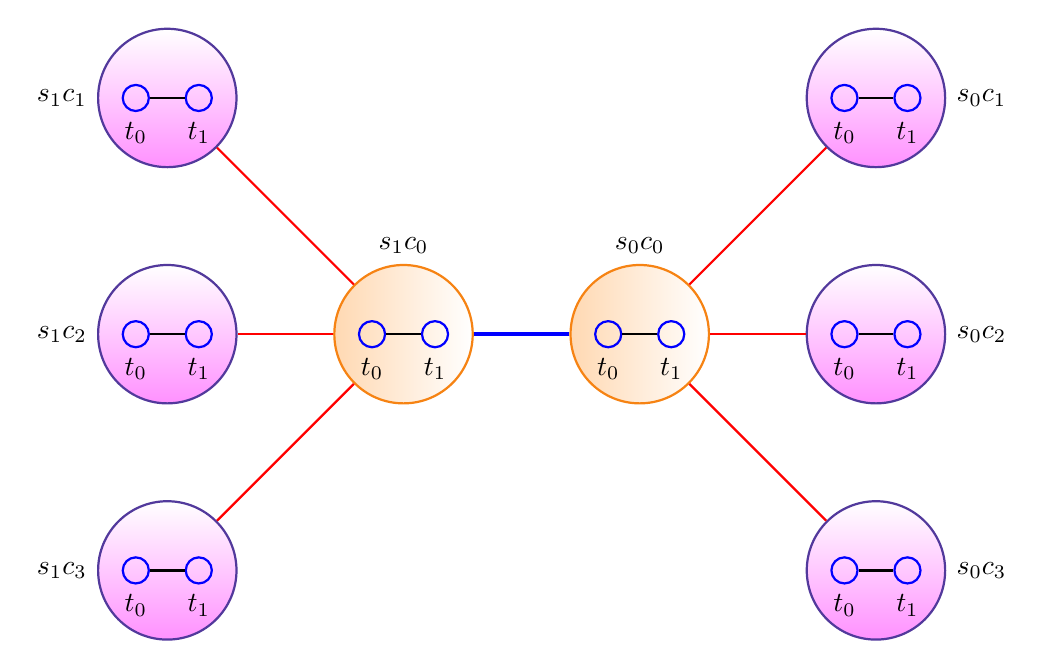
\begin{tikzpicture}[auto, thick]
  % Place base case
  \node[base,label=above:$s_0c_0$] (s0c0) at (1,0) {};
  \node[time,label=below:$t_0$] (s0c0t0) at (0.6,0) {};
  \node[time,label=below:$t_1$] (s0c0t1) at (1.4,0) {};
  
  \node[contingency,label=right:$s_0c_1$] (s0c1) at (4,3) {};
  \node[time,label=below:$t_0$] (s0c1t0) at (3.6,3) {};
  \node[time,label=below:$t_1$] (s0c1t1) at (4.4,3) {};

  \node[contingency,label=right:$s_0c_2$] (s0c2) at (4,0) {};
  \node[time,label=below:$t_0$] (s0c2t0) at (3.6,0) {};
  \node[time,label=below:$t_1$] (s0c2t1) at (4.4,0) {};

  
  \node[contingency,label=right:$s_0c_3$] (s0c3) at (4,-3) {};
  \node[time,label=below:$t_0$] (s0c3t0) at (3.6,-3) {};
  \node[time,label=below:$t_1$] (s0c3t1) at (4.4,-3) {};
  
  \path (s0c0t0) edge (s0c0t1);
  \path (s0c1t0) edge (s0c1t1);
  \path (s0c2t0) edge (s0c2t1);
  \path (s0c3t0) edge (s0c3t1);
  
  \path[cedge] (s0c0) edge (s0c1);
  \path[cedge] (s0c0) edge (s0c2);
  \path[cedge] (s0c0) edge (s0c3);

  % Second scenario
  \node[base,label=above:$s_1c_0$] (s1c0) at (-2,0) {};
  \node[time,label=below:$t_0$] (s1c0t0) at (-2.4,0) {};
  \node[time,label=below:$t_1$] (s1c0t1) at (-1.6,0) {};
  
  \node[contingency,label=left:$s_1c_1$] (s1c1) at (-5,3) {};
  \node[time,label=below:$t_0$] (s1c1t0) at (-5.4,3) {};
  \node[time,label=below:$t_1$] (s1c1t1) at (-4.6,3) {};

  \node[contingency,label=left:$s_1c_2$] (s1c2) at (-5,0) {};
  \node[time,label=below:$t_0$] (s1c2t0) at (-5.4,0) {};
  \node[time,label=below:$t_1$] (s1c2t1) at (-4.6,0) {};

  
  \node[contingency,label=left:$s_1c_3$] (s1c3) at (-5,-3) {};
  \node[time,label=below:$t_0$] (s1c3t0) at (-5.4,-3) {};
  \node[time,label=below:$t_1$] (s1c3t1) at (-4.6,-3) {};
  
  \path (s1c0t0) edge (s1c0t1);
  \path (s1c1t0) edge (s1c1t1);
  \path (s1c2t0) edge (s1c2t1);
  \path (s1c3t0) edge (s1c3t1);
  
  \path[cedge] (s1c0) edge (s1c1);
  \path[cedge] (s1c0) edge (s1c2);
  \path[cedge] (s1c0) edge (s1c3);

  \path (s0c0) edge [ultra thick,color=blue] (s1c0);

\end{tikzpicture}

\caption{Stochastic multi-period contingency constrained structure with two scenarios $s_0$ and $s_1$. Each scenario has three contingencies $c_1$,$c_2$,and $c_3$. $s_0c_0$ and $s_1c_0$ denote the base-cases for the two scenarios. Each scenario and contingency has two time-periods $t_0$, and $t_2$, $t_2$. The {\textcolor{red}{red}} line denotes the coupling between the contingencies and their respective base-case scenarios.The {\textcolor{blue}{blue}} line denotes the coupling between the scenarios}
\label{fig:sctopflow}
\end{figure}
